%!TEX TS-program = xelatex
%!TEX encoding = UTF-8 Unicode
% !TeX spellcheck = en_US

\documentclass[aspectratio=169]{beamer}
%%\usepackage{polyglossia}    
%%\setmainlanguage{english}
\usepackage[utf8]{inputenc}
\usepackage[T1]{fontenc}
\usepackage{ae,aecompl}
\usepackage{psfrag}
\usepackage{listings}
\usepackage{courier}
\lstset{basicstyle=\footnotesize\ttfamily,breaklines=true}
\usepackage{units}
\usepackage[official]{eurosym}
\usetheme{metropolis}           % Use metropolis theme
\usepackage{xspace}
\usepackage{qrcode}


\title{Angel Introduction: A/V Bunny}
\author{sophie \& jwacalex}
\institute{C3VOC}


\begin{document}

\maketitle


\begin{frame}{Agenda}
\tableofcontents
\end{frame}


\section{General Info}
\begin{frame}{General Info I}
	\begin{itemize}
		\item All talks get recorded and archived forever
		\item Consistent quality
		\item No postproduction of individual signals.
		\item Livestream content is the same as the one recorded and published
		\item Less mistakes $\Rightarrow$ better recordings.
	\end{itemize}
\end{frame}


\begin{frame}{General Info II}
	\begin{itemize}
		\item Introduction Meeting here
		\item Complete overview for all new angels
		\item Short update for experienced ones
	\end{itemize}
\end{frame}

\begin{frame}{General Info III}
Slides available online: \texttt{https://streaming.selfnet.de/engelschulung.pdf}

	\begin{figure} 
		\centering
		\qrset{link, height=5cm}
		\qrcode{https://streaming.selfnet.de/engelschulung.pdf}
	\end{figure}
\end{frame}

\section{Lecture Hall Operation}
\begin{frame}{A/V Bunny}
	\begin{itemize}
		\item An A/V Bunny is responsible for Audio and Video in a Lecture Hall\\
		$\Rightarrow$ They operate the audio mixer, the camera and the video mixer
		\item Also: Troubleshooting for A/V issues
		\item Also: A bit of stage management
		\item \textbf{Two} A/B Bunnies per talk $\Rightarrow$  Talk to your fellow bunnies about preferences
		\item in doubt: don't panic
	\end{itemize}
\end{frame}


\begin{frame}{Camera Operation}
	\begin{itemize}
		\item Operate the fixed cameras in the lecture halls
		\item Maintain good camera settings
		\item If necessary, readjust the camera
	\end{itemize}
\end{frame}

\begin{frame}{Video Mixer Operation}
	\begin{itemize}
		\item Switch the video feed between different sources. 
		\item Mixed video feed is used for both the live-stream and the recordings 
		\item You decide which picture, respectively source, is most interesting/important at each moment.
	\end{itemize}
\end{frame}



\section{Camera Hardware}
\begin{frame}{Hardware Camera Controls}
	\begin{columns}[T,onlytextwidth]
		\column{0.5\textwidth}
		\begin{figure} 
			\centering
			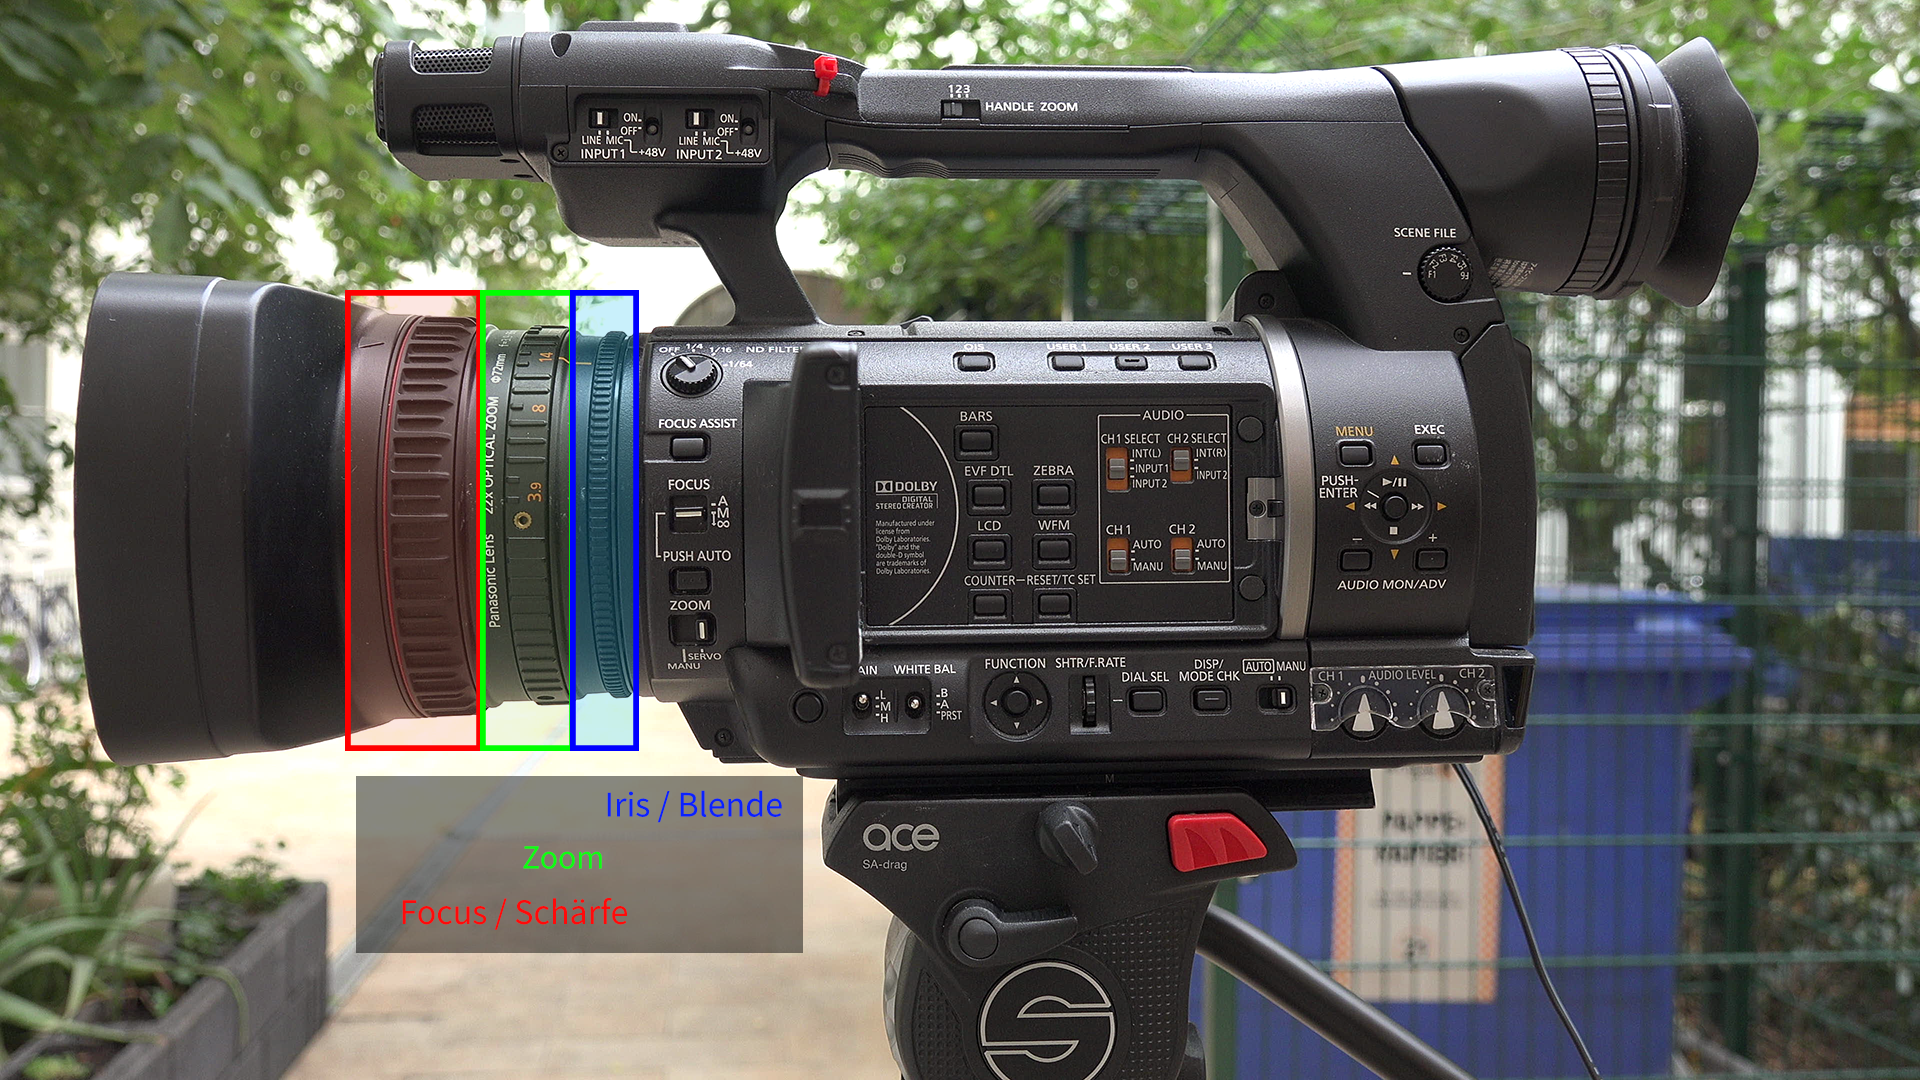
\includegraphics[width=0.9\textwidth]{images/panasonic_seitenansicht_objektiv.png}
			%\import{images}{camera-controls.pdf.tex}
			\caption{Camera Controls}
		\end{figure}
		\column{0.5\textwidth}
		Cameras are in manual mode because of difficult lighting situation.
		\begin{description}
			\item[Left Ring] Focus - control sharpness of the image.
			\item[Middle Ring] Zoom - vary the focal length.
			\item[Right Ring] Iris - don't touch.
		\end{description}
	\end{columns}
\end{frame}

\begin{frame}{Tripod Handle Controls}
	\begin{columns}[T,onlytextwidth]
	\column{0.5\textwidth}
	\begin{figure} 
		\centering
		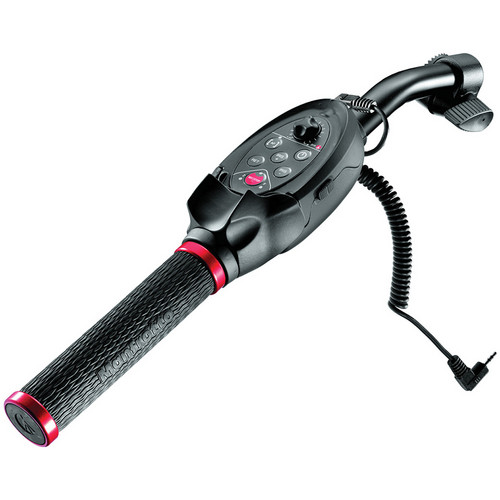
\includegraphics[width=0.7\textwidth]{images/tripod-handle.jpeg}
		\caption{Tripod Handle}
	\end{figure}

	\column{0.5\textwidth}
	Beware: various models in use.
	\begin{description}
		\item[Zoom Control] lever above red ring
		\item[Red Button] Start/stop recording, don't touch
		\item[Other Buttons] markings on the handle
    \end{description}

	\end{columns}
\end{frame}

\begin{frame}{Tripod}
	\begin{columns}[T,onlytextwidth]
	\column{0.4\textwidth}
	\begin{figure} 
		\centering
		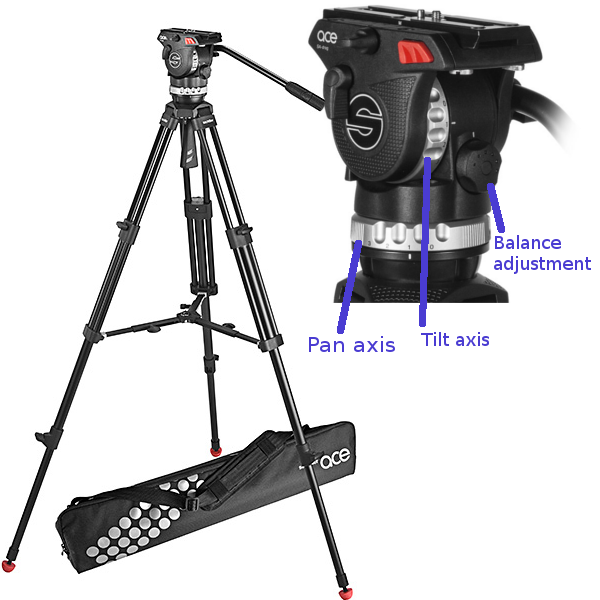
\includegraphics[width=0.9\textwidth]{images/tripod-complete.png}
		\caption{Tripod}
	\end{figure}
	
	\column{0.6\textwidth}
	\begin{itemize}
			\item Should be level - check the water bubble.
			\item Variable brakes - can be adjusted to your needs.
			\item Tilt axis should be balanced, so that the camera doesn't tilt up or down on its own.
			\item Pan axis is needed all of the time. Set it so you can do smooth pans all over the stage.
		\end{itemize}
	\end{columns}
\end{frame}

\begin{frame}{SD-Card Recording}
		\begin{itemize}
			\item Two SD-Cards in one camera each room
			\item Backup Recording
			\item Turn on Recording before first shift in the morning -> Red Dot somewhere in the Display.
			\item Control Recording Time remaining. 
		\end{itemize}
		\metroset{block=fill}
\end{frame}


\section{Video Mixer Tools}
\begin{frame}{Software Video Mixer - Controls}
	\begin{columns}[T,onlytextwidth]
	\column{0.5\textwidth}
	\begin{figure} 
		\centering
		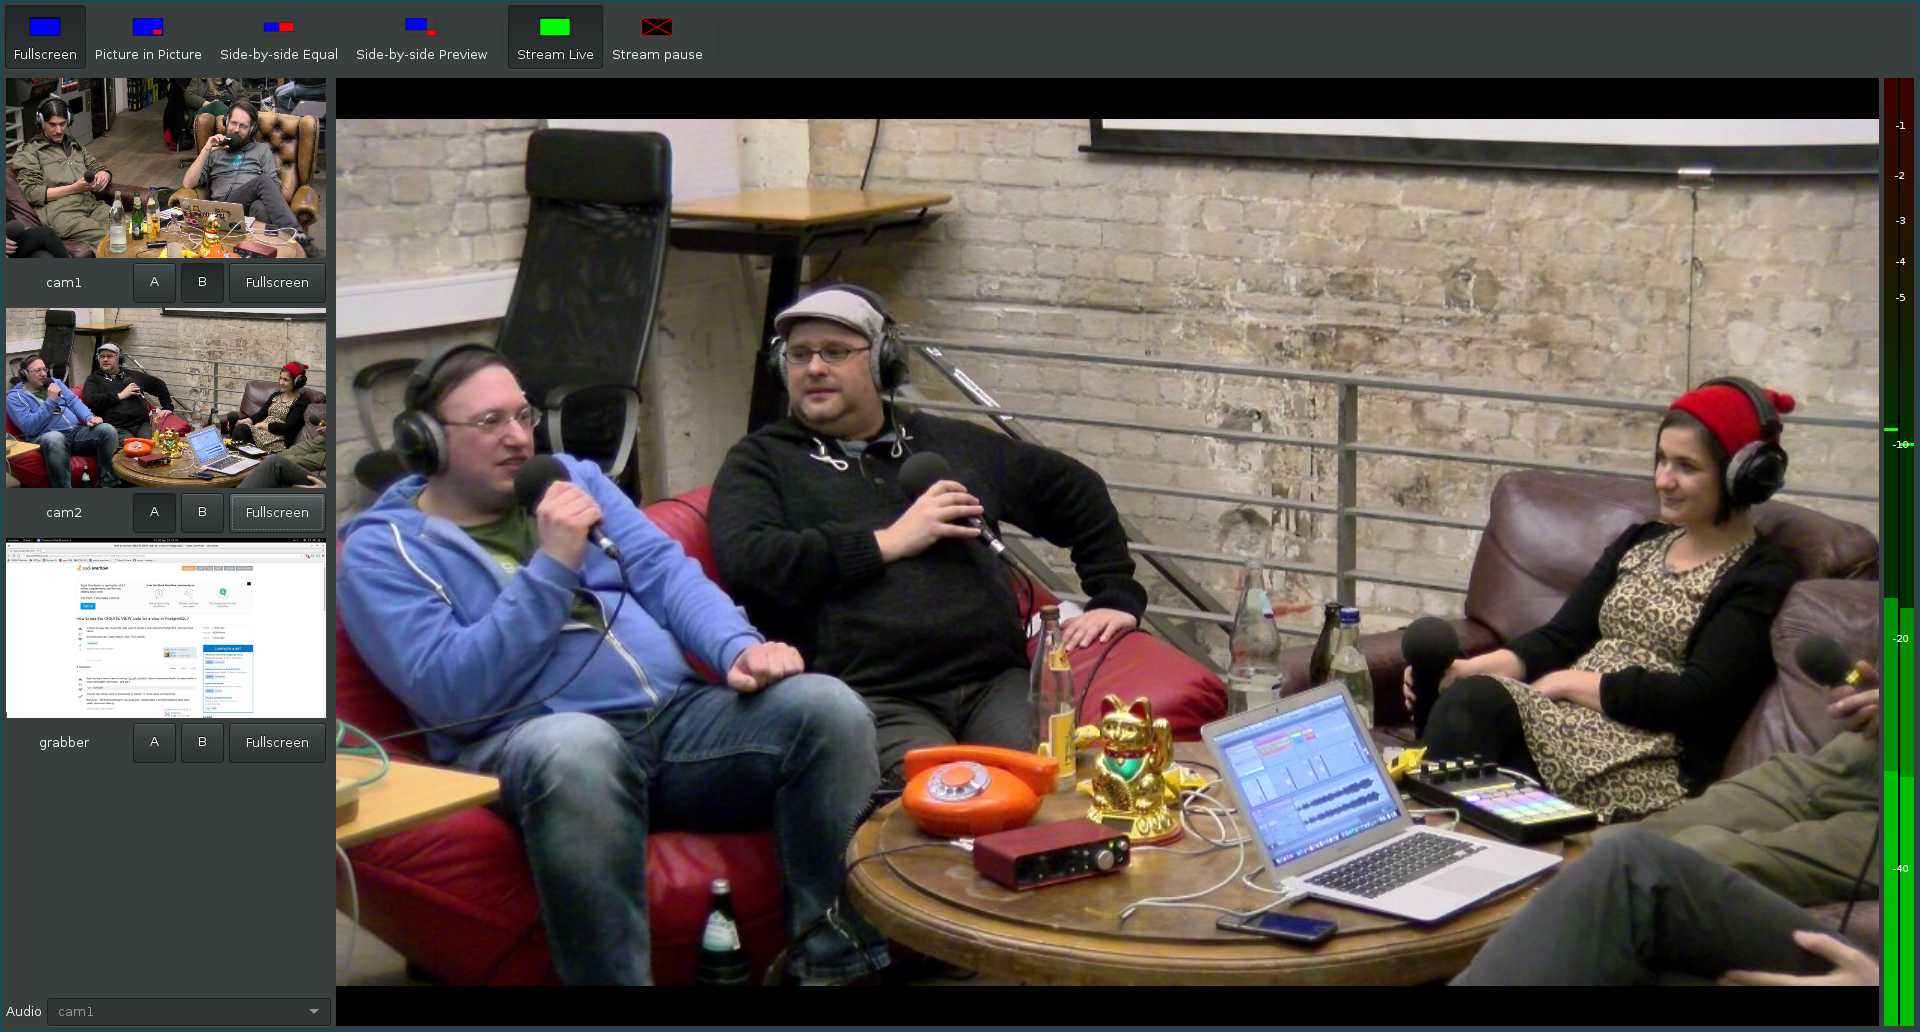
\includegraphics[width=1\textwidth]{images/voctomix.png}
		\caption{Voctogui}
		\label{fig:voctogui1}
	\end{figure}

	\column{0.5\textwidth}
	\begin{description}
		\item[Previews] Small images on the left 
		\item[Program] Large, middle, what everyone on the internet sees.
		\item[Composition] Top row.
		\item[Blue] Select A
		\item[Red] Select B
		\item[Stream Blank] For breaks when nothing should be streamed.
     \end{description}
	\end{columns}
\end{frame}

\begin{frame}{Software Video Mixer - Voctogui}
	\begin{figure} 
		\centering
		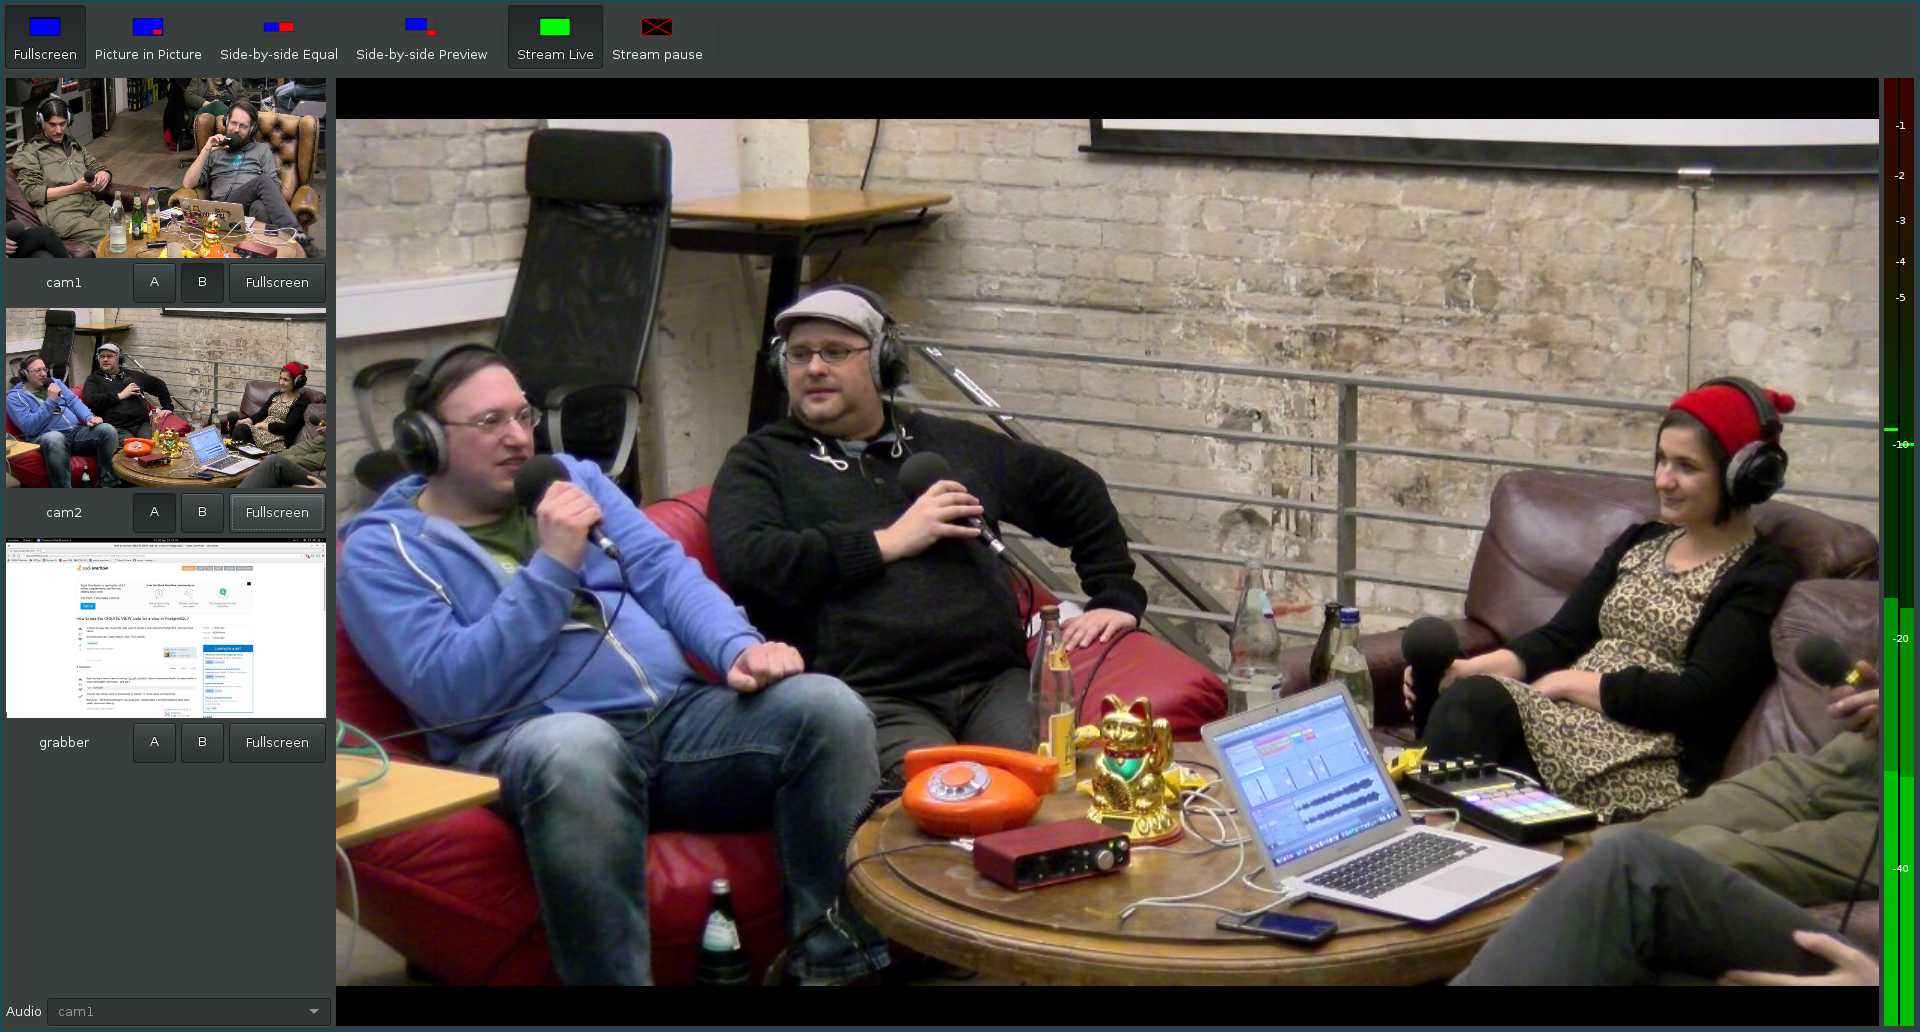
\includegraphics[width=.9\textwidth]{images/voctomix.png}
		\caption{Voctogui}
	\end{figure}
\end{frame}

\section{Video Mixing Guidelines}
\begin{frame}{Mixing Guidelines - Hard Rules}
	\begin{itemize}
		\item \textbf{All} you are doing is \textbf{recorded} and will be published. \alert{\textbf{Don't make mistakes.}}
		\item The Audience is \textbf{not to be filmed}. Cut away if faces of people not on the stage appear.
		\item \textbf{Slides are important}
		\item Slides stay on till the text has been read \textbf{twice}.
		\item Show new slides \textbf{immediately}.
	\end{itemize}
	\begin{exampleblock}{Hint}
		Fast-paced presentations with lots of slides are easier to handle with the supersource.
	\end{exampleblock}
\end{frame}


\begin{frame}{Mixing Guidelines - Softer Hints}
	\begin{itemize}
		\item Start early – opening announcements of the Herald are a good start. Their introduction has to be in the recording and on stream.
		\item Open wide – Structure the beginning of a talk with shots that set the stage
		\item The slides in fullscreen – you’re dealing with a very small screen. Text has to be readable
		\item Show gestures – medium-close-up that follows the speakers eye-line
		\item Don’t be too cutty – Pace your videos temperately. Do not cut too often.
		\item Don't end too early – All questions and answers have to be recorded. The herald ends the talk, not the mixer angel.
	\end{itemize}
	\begin{exampleblock}{Hints}
		Leave lots of room at the start and end of a talk. 
		Cut away from the infobeamer before the Herald starts with announcements. 
		Cut to the infobeamer only after the last applause has finished.
	\end{exampleblock}
\end{frame}

\section{Timeline of a Talk}

\begin{frame}{Timeline of a typical talk}
	\begin{enumerate}
		\item Preparations beforehand
		\item Announcements and Introduction
		\item Content
		\item Questions and Answers
		\item Ending
	\end{enumerate}
\end{frame}

\begin{frame}{Timeline - Preparations beforehand}
	\begin{block}{Cameras}
		\begin{itemize}
			\item Get to know your fellow angels.
			\item Test your camera and settings.
			\item Camera: Get a closeup of the speaker or their movement
		\end{itemize}
	\end{block}
	\begin{block}{Mixer}
		\begin{itemize}
			\item Check Slides and adjust supersource to 16:9 or 4:3.
		\end{itemize}
	\end{block}
	\begin{block}{Audio}
	\begin{itemize}
		\item Setup the Headset(s) and Mic for audience question
		\item Perform a short sound check
		 \item Adjust the levels
	\end{itemize}
\end{block}
\end{frame}

\begin{frame}{Timeline - Announcements and Introduction}
	
	\begin{block}{Mixer}
		\begin{enumerate}
			\item Go live with Camera as soon as the talk starts.
			\item Title slide can be shown during the introduction 
			\item Put Camera  on Preview.
			\item Camera live as soon as the Speaker starts talking
		\end{enumerate}
	\end{block}
\end{frame}

\begin{frame}{Timeline - Content}
	\begin{block}{Cameras}
		\begin{itemize}
			\item Look for time to time if you have to readjust zoom, focus or anything else that should not be in the recording.
			\item Prior makeing adjustments, ensure that the camera is not live
		\end{itemize}
	\end{block}
	
	\begin{block}{Mixer}
		\begin{itemize}
			\item Show new slides as soon as they are keyed by the Speaker 
			\item Call out your actions and intentions via intercom
			\item Plan ahead. Which picture should be shown in 30 seconds?
		\end{itemize}
	\end{block}

	\begin{block}{Audio}
		\begin{itemize}
			\item Monitor audio levels and adjust if the speaking person is too loud/too silent
		\end{itemize}
	\end{block}

\end{frame}

\begin{frame}{Timeline - Questions and Answers}
	\begin{block}{Cameras}
		\begin{itemize}
			\item Keep tracking the speaker, don't give up even if your shift ends soon.
		\end{itemize}
	\end{block}
	
	\begin{block}{Mixer}
		\begin{itemize}
			\item Show whoever is talking on stage to the stream.
			\item The "Thanks"-Slide can be shown from time to time.
			\item Don't end too early.
		\end{itemize}
	\end{block}

	\begin{block}{Audio}
	\begin{itemize}
		\item Unmute question mic 
			\item Monitor audio levels and adjust if the speaking person is too loud/too silent
	\end{itemize}
\end{block}
\end{frame}

\section{Orga} 		
\begin{frame}{Shift Distribution}		% Alex
\begin{itemize}
	\item Video Mixer shifts will be distributed in the angel system
	\item Sign up to the shifts you want to take
	\item Talks with special requirements might be handled by VOC
\end{itemize} 
\end{frame}
% mündlich: 	\item Everyone should do at least one shift per day

\subsection{Contacts}			% Alex
\begin{frame}{Who to Contact?}
\begin{itemize}
	\item General Issues - VOC \textbf{1600}
	\item Organizational or social problems 
	\begin{itemize}
		\item sophie - DECT  \textbf{7425}
		\item jwacalex - DECT \textbf{5523}
	\end{itemize}
	\item We might need to call you. Please have your DECT (or UMTS) number in the Engelsystem! If you don't have a number yet, go to 
	\textcolor{blue}{\textbf{eventphone.de}} and get one. 
\end{itemize} 
\end{frame}

\begin{frame}{Questions?}
Contact us in our office or via irc, \#voc-lounge on hackint.
\end{frame}

\end{document}


%%% End
